%!TEX root = ../main.tex
\documentclass[a4paper,oneside,12pt, class=Latex/Classes/PhDthesisPSnPDF, crop=false]{standalone}
\usepackage{setspace}
\begin{document}
\doublespacing
\chapter{Introduction}
\label{chap:intro}

\section{The final stages of stars}
Stars are big balls of plasma that is gravitationally bound together. Consisting of primarily hydrogen upon first formation, the extreme heat and pressure in their cores allows stars to fuse hydrogen into helium, which generates the energy needed to maintain hydrostatic equilibrium and prevent further gravitational collapse. \citet{starstruct} gives an excellent and detailed review of the evolution of stars in different mass ranges. When the hydrogen supply is depleted the inward pressue from gravity causes the core to contract until something is able to stop it once more. This can be matter in the core turning degenerate and providing an electron degeneracy pressure, or the start of helium fusion. What happens next, and the ultimate fate of a star depends on its mass.


\subsection{Stars below 8 M$_\odot$}
\label{interm_mass_stars}
The lightest stars have a theoretical lifespan that is larger than the current age of our universe, and as such the final stages of their evolution cannot be observed yet. The outer layers of stars with a mass between 0.6 M$_\odot$ and 8 $M_\odot$ increase dramatically, and they become red giants as they fuse helium into carbon and oxygen in their cores and hydrogen in a shell around the core. Eventually the outer layers are blown away while the core is left behind to cool down and become a white dwarf (WD).

WDs are degenerate objects primarily made up of carbon and oxygen. As electrons are fermions, the Pauli exclusion principle \citep{Pauli} forces each one to occupy a different quantum state. Due to their high density in the WD, electrons become degenerate as they are forced in higher energy states. The degenerate electron gas provides a pressure that is independent of temperature, allowing the WD to theoretically cool to absolute zero without any significant change in the stellar structure (although some models predict WDs to crystallise at a certain temperature, \citealt{WD_crystal_Mochkovitch, WD_crystal_Isern}). Assuming that the electron gas is non-relativistic, it can be shown that the radius of a WD is related to its mass as

\begin{equation}
    \label{nonrel_WD_eq}
    \frac{R_\text{WD}}{R_\odot} = 0.010 \left(\frac{M_\odot}{M_\text{WD}}\right)^{1/3},
\end{equation}

with $R_\text{WD}$ the radius of the WD and $M_\text{WD}$ its mass. This shows that WDs are roughly planet sized, and that more massive WDs are smaller. As the mass increases however, the electrons in the WD become relativistic and Equation~\ref{nonrel_WD_eq} is no longer valid. In this case the radius decreases much more drastically with increasing mass, up to the limit of 

\begin{equation}
    \label{Chandrasekhar_lim}
    M_\text{Ch} \approx 1.4 M_\odot,
\end{equation}

which is the so-called Chandrasekhar limit \citep{Chandrasekhar_lim}. A WD at the Chandrasekhar mass $M_\text{Ch}$ has a radius of 0, and the electron degenerate pressue cannot stop a WD from collapsing in on itself.


\subsection{Stars above 8 M$_\odot$}
\label{ge_8_Msol}

\begin{figure}
    \centering
    \includegraphics[width=\textwidth]{../Images/chapter_1/starstruct.png}
    \caption{Schematic view of the onion structure of a highly evolved massive star just before core collapse, with light elements on the outside and heavier elements towards the core. Typical values are given along the horizontal and vertical axes. This figure originally comes from chapter 35 of \citet{starstruct}.}
    \label{startstruct}
\end{figure}

More massive stars are able to burn the carbon that is left after burning helium. New elements get created and subsequently burned under increasingly more extreme conditions, resulting in a core which is structured like an onion. Each ring consists of a different fusion product, with heavier elements towards the core. Figure \ref{startstruct} shows a schematic view of the layered structure of a highly evolved massive star. Each stage of fusion is less efficient, and once iron is reached it further fusion consumes energy rather than releasing it. The core becomes unstable to support itself and collapses into a neutron star or black hole, depending on the mass of the star. The outer layers fall inwards but bounce back and gains enough energy to become unbound from the star. Additionally the high densities allow for elements heavier than iron to be fused in these brief moments. The stellar demise is known as a core collapse supernova (CCSN). Section \ref{CCSN} contains more details on these events.


\section{The transient universe}
Astronomy is a field filled with large scales, and when studying processes that change over time our limited time-span to observe often prevents us from studying a single object through its entire evolution. From formation of stars and planets to the the evolution of galaxies and the cosmic web, these occur on such long time scales that a human life is just a blip. From our perspective we only have a snapshot of the state of each object, and it is through the combination of a large ensemble of objects together with theory and simulations that we are able to understand the bigger picture.

Transients are, by definition, fleeting things, and in extrasolar astronomy these are objects or events that occur on short timescales of mere hours to a few years. This means we are able to observe the entire evolution of a single object, as long as it is discovered early. The most famous examples of transients are supernovae (SNe), exploding stars at the end of their life releasing enough light that they can outshine their entire host galaxy for a few weeks to months before fading away again.

Figure \ref{2024gy_ZTF} is a \ztfg\ztfr\ztfi\ composite image of NGC4216, taken with the Zwicky Transient Facility (ZTF, see Section \ref{ZTF}). The left image is made using data before the start of 2024, the right image is made using data from Januari 2024 and clearly shows an extra source in the southern part of the galaxy. This is SN 2024gy, a Type Ia SN (see Section \ref{SNIa}) first discovered on 4 Jan 2024 \citep{2024gy_disc}. Despite the galaxy being at a distance of $16.194 \pm 0.491$ Mpc \citep{2024gy_z} the SN still outshines the Milky Way stars that are in the same image.

\begin{figure}
    \centering
    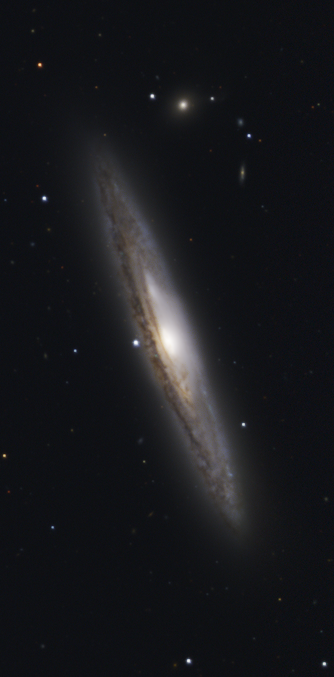
\includegraphics[width=0.49\textwidth]{../Images/chapter_1/SN2024gy_pre-SN.png}
    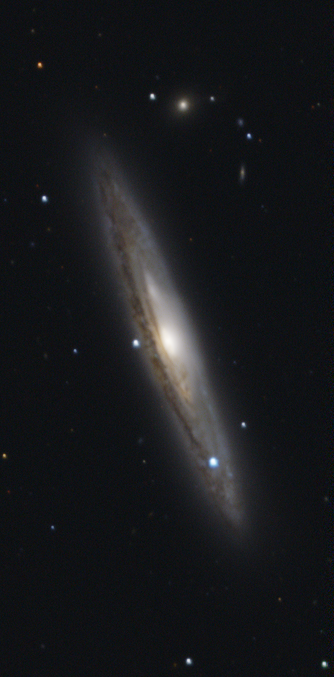
\includegraphics[width=0.49\textwidth]{../Images/chapter_1/SN2024gy_active.png}
    \caption{\ztfg\ztfr\ztfi\ composite image of NGC4216 using observations taken by the Zwicky Transient Facility. \textbf{Left:} composite image of observations taken before 1 January 2024. \textbf{Right:} composite image of observations taken between 5 and 19 January 2024, the first two weeks after the first detection of the Type Ia SN~2024gy. (Credit: Benjamin Nobre Hauptmann)} %30, 29, 14 (gri sn images) & 35, 31, 30 (gri pre-SN images) given to Benjamin, subset used based on data quality, exact numbersnot so relevant
    \label{2024gy_ZTF}
\end{figure}


\subsection{Core Collapse Supernovae}
\label{CCSN}
As was mentioned at the end of Section \ref{ge_8_Msol}, stars above 8 $M_\odot$ end their lives in a CCSN when the core implodes into a compact object due to the effects of gravity. The outer layers fall in as well but bounce back outwards as the enormous amounts of released gravitational energy from the collapsing core is imparted on the outer layers, heating them up and expelling them outwards at high velocities. The light coming from the cooling of this material and the radioactive decay of newly formed unstable nuclei into stable ones cause the SN to rise rapidly in brightness. Within hours after the explosion it is bright enough to be observed in other galaxies, peaking after several days to weeks at an absolute magnitude in the range of -16.5 Mag to -18.5 Mag depending on the type of CCSN \citep{SN_M_dist}. This is what we observe as the supernova event, and by analysing their spectra they can be classified based on the visble elemental emission and absorption lines.

The composition of the outer layers of the progenitor star depend heavily on the life of the star. Most CCSNe have hydrogen in their envelope, which will show up in the SN spectra as strong Balmer emission lines. These are known as Type II SNe. Photometric features of the light curve, the SN brightness as it changes over time, are also used in SN identification, leading to subtypes such as SN IIL or SN IIP for Type II SNe that show a linear decline or a plateau, respectively. High mass-loss rates, due to the stars metallicity or the presence of a binary companion, can however strip the hydrogen layer leaving the helium shell as the outermost part of the progenitor at the moment of core collapse which results in a SN without H lines but with He lines in their spectra that are known as Type Ib SNe. In some extreme cases even the helium layer has been stripped away, resulting in SNe without H or He lines in their spectra, known as Type Ic SNe. Transistional objects, where a layer is mostly but not completely stripped, are also known \citep{SN_large_pic}.

Photometric classification is cheaper as photometry is easier to obtain, but it cannot differentiate between subtypes that are defined on the presence, strength, or absence of specific elemental lines, leading to broader classifications with less certainty. Besides this, many of the differences that make certain SNe interesting are visible at early times, while a SN needs to evolve up to a certain point to have a light curve that is long enough to allow classification. For these reasons a common strategy is to use dedicated large-scale surveys such as the Zwicky Transient Facility (ZTF, see Section \ref{ZTF}) to find new SNe within days after explosion using photometry, and using different telescopes to follow these up with spectroscopy for classification.

\subsection{Thermonuclear SNe}
\label{SNIa}
Besides CCSNe are the more common thermonuclear SNe (Type Ia SNe, SNe Ia), which are exploding WDs after fusion in their core has been ignited through some mechanism (see Section \ref{Ia_progenitors}). The more massive the WD, the easier it is to ignite as the nuclei are forced closer together. Since the WD is degenerate the energy released by a single fusion event can completely be used to heat up the surrounding material and let it fuse as well, leading to a runaway process where the entire WD tries to fuse to iron-peak elements on a timescale of seconds. This process disrupts the entire star, expelling the material outward at relativistic speeds \citep{Ia_thermonuclear}. Not all carbon and oxygen is fused, but most of the mass ends up in $\Nififtysix$, with typical SNe Ia producing between 0.3 -- 0.8 $M_\odot$ of $\Nififtysix$ \citep{Ia_Ni56_yield}. This is an unstable nucleus and decays as
\begin{equation}
    \Nififtysix\ \xrightarrow{6.1\text{ d}}\ \Cofiftysix\ \xrightarrow{77.3\text{ d}}\ \Fefiftysix,
\end{equation}
with $\Fefiftysix$ being the stable end product of the decay chain. The key spectral signatures of a SN Ia are the absence of hydrogen lines (hence the Type I classification), and broad \SiII\ absorbtion features. At first the ejecta are dense and opaque, and only photons from the outer layers can escape. As the ejecta expand they become more transparent, and the slower moving inner layers become visible as the photosphere recedes back inwards. Therefore, by taking spectra at different phases a map of the elemental abundances in velocity space can be built. \color{red}Rewrite the spectra part, doesn't feel right, needs refs \color{black}

The SN reaches peak brightness around three weeks after the explosion and starts to fade again. The main powersource that governs the rate at which the SN fades is the decaying $\Nififtysix$, resulting in a linear decline of the light curve in magnitude space. In the near infrared there is a second peak a few weeks after the first, which is suggested to be the result of a decrease in opacity due to the changing ionization state of iron group elements \citep{2nd_max}. Figure \ref{Ia-norm_example} shows an example of a well-observed normal SN Ia.

\begin{figure}
    \centering
    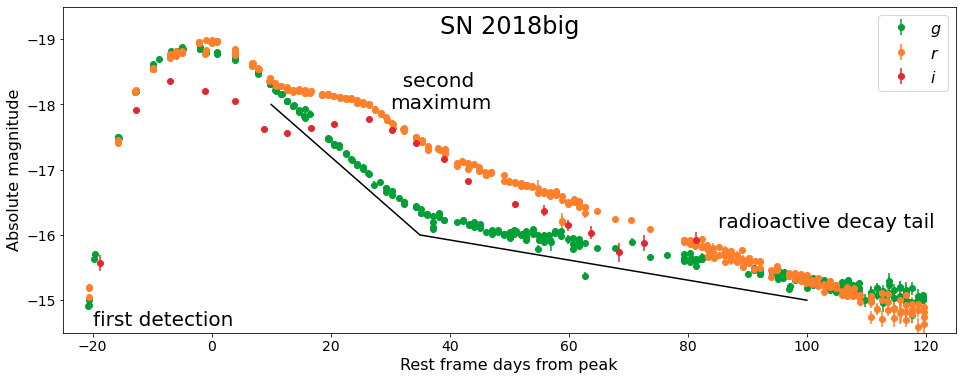
\includegraphics[width=\textwidth]{../Images/chapter_1/Ia-norm_example.png}
    \caption{\ztfg\ztfr\ztfi light curve of a SN Ia in the rest frame and at absolute magnitude, corrected for Milky Way extinction but not for host extinction. The \ztfg-band clearly shows a change in the decline rate as $\Cofiftysix$ decay becomes dominant over $\Nififtysix$ decay. The \ztfr\ and \ztfi-band show the second peak. This light curve is made using ZTF observations.}
    \label{Ia-norm_example}
\end{figure}

\subsubsection{Standardizable candles}
\label{Standard_candle}
A WD with a mass of $\sim 1.37 M_\odot$ has high enough pressure and density in its core for carbon to ignite, triggering a thermonuclear runaway process that results in the SN Ia explosion. Most WDs tend to explode in a very similar way, which results in very similar light curves that peak around an absolute magnitude of -19.5 Mag, making them brighter than CCSNe. Some SNe Ia become brighter than others, but they also evolve slower. This is called the Phillips relation \citep{phillips_rel}, and it can be used to infer the absolute peak brightness based on how fast it evolves. \citet{Tripp_colour_rel} improved the standardization by adding a second term, the so called colour luminosity term. This accounts for the intrinsic SNe Ia colour and as bluer SNe Ia are brighter. These days there is a third term, which accounts for environmental dependencies and is implemented as a step function \citep{Kelly_mass_step, Sullivan_mass_step}. The resulting standardisation formula is given by
\begin{equation}
    \mu_\text{obs} = m_B - M_0 + \alpha x_1 - \beta c - \gamma p,
\end{equation}
where $\mu_\text{obs}$ is the observed distance modulus. $m_B$ and $M_0$ are the apparent and absolute B-band magnitude, respectively. $x_1$ is the SN stretch, $c$ its colour, and $\alpha$ and $\beta$ are the coefficents used to correct for these effects. $\gamma$ is the size of the step function and $p$ determines when this step needs to be applied.

Using the standardisable nature of SNe Ia allows their distance to be measured, as well as the distance between Earth and the host galaxies they reside in. At the same time the redshift of the host galaxy can be measured from the spectra, and with these values together the Hubble constant $H_0$, wihch measures the expansion rate of the universe, can be measured. According to one of the latest measurements made by the SH0ES team \citep{SH0ES} using the Pantheon+ sample \citep{Pantheon+} the universe expands at a rate of $H_0 = 73.30 \pm 1.04$ km s$^{-1}$ Mpc$^{-1}$.


\subsection{Other types of transients}
There are other types of transients besides SNe. Some SNe become much brighter than normal events and are therefore called superluminous SNe (SLSNe). Supermassive black holes (SMBHs) in the center of galaxies can cause a variety of transient events such as tidal disruption events (TDEs) or ambiguous nuclear transients (ANTs), or a galaxy could have an active galactic nucleus (AGN). Some types of stars also pulsate and vary in brightness over time. All of these can show up transients in surveys looking for changes in the night sky on a day-to-day basis.


\subsubsection{SLSN - Superluminous Supernova}
SLSNe are SNe that have a higher peak luminosity than normal SNe, in some cases reaching over 5 magnitudes brighter than normal events at their peak \citep{SLSN_Gal-Yam}. Like normal SNe they can be classified into Type I and Type II based on the absence of presence of hydrogen emission lines in their spectra. One of the main puzzles regarding these types of events is the source that powers their superluminous nature. Different types of models have been put forward, using magnetars \citep{Maeda_SLSN_magentar}, black holes \citep{SLSN_BH}, radioactivity \citep{Kasen_SLSN_pair_instab}, or interaction with circumstellar material (CSM) \citep{Late-time_CSM_SLSNE_I} to push the brigthness significantly above that of regular SNe. Each of these has different strengths and weaknesses.


\subsubsection{AGN - Active Galactic Nucleus}
An AGN is the central region of a galaxy in which a SMBH accretes matter at a high rate, releasing a part of the potential energy as heat and radiation. As a result of this the AGN has a very high luminosity compared to the rest of the galaxy, with different orientations of the system resulting in different types of AGN \citep{Antonucci_1993_AGN, Urry_1995_AGN}. As the stream of matter being accreted is inhomogeneous, the accretion rate and luminosity change over time. In some cases AGN variability is so extreme that it changes the entire spectrum of the AGN, with (dis)appearing broad emission lines and continuum flux. These are so called changing-look AGN (CL-AGN) \citep[see][for a review]{CLAGN}. AGN variability can be used to estimate the SMBH mass through reverberation mapping \citep{Reverberation_mapping, Reverberation_Peterson}. Fast moving clouds close to the AGN change the strength of line emission based on how strongly they are illuminated by the AGN. The delay between a luminosity change in the AGN continuum and the broad emission line features coming from these clouds gives a measure of their distance, while the width of the emission lines give a measure of their velocity. From these measurements the SMBH mass can be estimated using Kepler's third law.


\subsubsection{TDE - Tidal Disruption Event}
In some cases a star can get too close to the SMBH and get tidally disrupted \citep{Rees_1988_TDE, Strubbe_2009_TDE}. In a TDE the star gets ripped apart due to the strong gravity of the SMBH and forms an accretion disk of hot gas that gets accreted onto the SMBH. The distance at which the TDE occurs depends largely on the SMBH mass, and for SMBHs more massive than $\sim10^8 M_\odot$ the tidal disruption radius lies within the event horizon, meaning that TDEs cannot be observed around the most massive SMBHs \citep{Hills_mass}. The other dependency of the tidal radius is the difficulty to disrupt a star. Compact objects such as WDs are very difficult to disrupt and thus have a smaller tidal radius. A red giant on the other hand has outer layers that are very loosely bound to the star and is therefore easier to disrupt at a larger radius, though this might also result in a partial tidal disruption where only the outer layers are stripped while the stellar core survives the encouter. TDEs can become brighter than SNe, with the brightest event ever observed being AT 2021lwx (ZTF20abrbeie, nicknamed "Scary Barbie"), which is thought to be the disruption and accretion of a giant molecular cloud \citep{Scary_Barbie, 2021lwx_Wiseman}.


\subsubsection{ANT - Ambiguous Nuclear Transient}
 Some nuclear variability does not quite fit the known classes of AGN or tidal TDEs, showing characteristics of both types of events. These events have been named ambiguous nuclear transients \citep[ANTS;][]{Kankare_ANT, 2020ohl_Hinkle, Hinkle_MIR_ANT_echo, Hinkle_Extreme_nuclear_transients/ANTs, wiseman_ztfants} and rise up quickly, reaching peak brightness within a few weeks before declining very slowly over hundreds of days, although their decline rates are variable. 


\subsubsection{Variable stars}
Some stars show variability as well, with the brightness of certain types of stars oscilating by a magnitude or more. The most famous class of variables are Cepheids, whose regular oscilation period of the order of days is related to their absolute magnitude. They are bright enough to be visible in nearby galaxies, which makes them useful to calibrate SN Ia distance measurements when building the distance ladder \citep{Cepheids_Gibson, Cepheids_Saha}. Other types of stars, such as Mira variables, are much more extreme in their change of brightness and have periods $>100$ days \citep{Mira_varibs}.


\section{SN Ia progenitor systems}
\label{Ia_progenitors}
Section \ref{interm_mass_stars} states that WDs are stable objects, but Section \ref{SNIa} states that WDs explode in SN Ia explosions. These two satements seem to disagree with each other, as a stable object is not expected to suddenly explode. This observation is correct, WDs do not explode. At least, not by themselves. However, not all stars are single, and those that in a binary system can under certain conditions interact with the other star and start accreting matter coming from the so-called donor star. As the radius of a WD is inversely proportional to its mass (Equation \ref{nonrel_WD_eq}), it will shrink as it becomes more massive until the point is reach where fusion is ignited in the core of the WD triggering its explosion.

The obvious thing to do is to ask what kind of star the donor is. Assuming that the stars have been in the binary system since formation and since more massive stars have a shorter lifespan, the more massive star has turned into the WD. This means that the donor has to be $<8$ $M_\odot$ (though due to stellar and especially binary evolution the mass of the donor has likely changed since formation). Other than this there are many possible options, the donor could still be in its hydrogen burning phase or have evolved to the later stages in its life up to and including becoming a WD as well. This is called the progenitor problem, and it is currently still being debated. Different progenitor scenarios can broadly be put into one of two categories base on whether the donor star is a compact object (double degenerate) or not (single degenerate). Artistic impressions of these two scenarios are shown in figure \ref{single_double_deg_mods}.

\begin{figure}
    \centering
    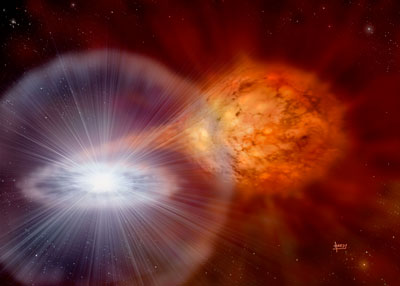
\includegraphics[height=0.229\textheight]{../Images/chapter_1/single_deg.jpeg}
    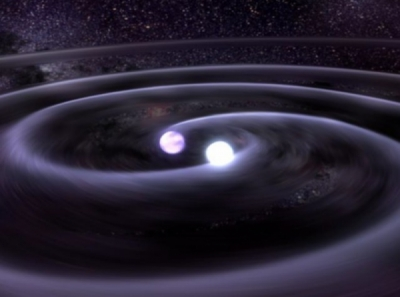
\includegraphics[height=0.229\textheight]{../Images/chapter_1/double_deg.jpeg}
    \caption{\textbf{Left:} Artistic impression of a single degenerate system, where the white dwarf accretes material coming from the surface of the donor star. Image credit: STFC / David Hardy. \textbf{Right:} Artistic impression of a double degenerate system where two white dwarfs spiral in to each other while releasing gravitational waves. Image credit: NASA / Tod Strohmayer (GSFC) / Dana Berry (Chandra X-Ray Observatory).}
    \label{single_double_deg_mods}
\end{figure}


\subsection{Single degenerate}
The most straightforward and classical way to explode a WD is by adding mass to a near $M_\text{Ch}$ WD until carbon is ignited in the core due to compressional heating. The companion star fills its Roche lobe and material from the outer layers is syphoned onto the WD. The donor can fill its Roche lobe while it is still a main sequence star, when it has evolved into a red giant, or it may even be a helium star whose hydrogen layer has been stripped due to binary interactions \citep{Whelan_classical_Ia_mod, Nomoto_single_degenerate}. In delayed-detonation models the WD first expands during a deflagration phase, which then transition into a detonation after the WD becomes unbound \citep{Kholov_Del_det, Mazzali_common_mechanism}.

In non-classical models a sub-$M_\text{Ch}$ WD can explode by first slowly accreting and building up a layer of helium on its surface, which explodes after a sufficient amount of material is gathered. As this explosion wraps around the outside of the WD it sends a shockwave into the interior of the star, which culminates near the center and temporarily increases the local pressure. If this is enough to ignite carbon fusion, the second detonation is triggered which disrupts the star and results in the main SN \citep{Taam_ddet, Livne_ddet, Shen_ddet, Fink_ddet}.

It is also possible that the WD and red giant companion enter a common envelope phase. The WD mergers with the hot core of the red giant forming a rapidly rotating, WD-like degenerate core with $M_\text{core}>M_\text{Ch}$ inside the red giant. The angular momentum prevents the core to collaps in on itself but is gradually lost until it can no longer support itself, triggering the SN Ia explosion in the so-called core degenerate scenario \citep{Kashi_core_deg}.


\subsection{Double degenerate}
If both objects are WDs the primary (more massive) WD can still accrete material from the secondary WD in a stable Roche lobe overflow scenario \citep{CO_accretion_I, CO_accretion_II}. In other scenarios the WDs fully merge, either dynamically or violently. In the dynamical scenario the WDs lose angular momentum as it is radiated away through gravitational waves \citep{Iben_Double_degenerate, Webbink_Double_degenerate}. An artist impression of this scenario is given on the right side of figure \ref{single_double_deg_mods}. As the WDs come closer the less massive companion fills its Roche lobe and material starts flowing onto the primary. As the companion loses mass its radius increases, leading to more mass loss until the entire star is disrupted. Around half of the material forms a disk around the surviving WD while the rest falls directly onto its surface, very little material is expected to be flung out of the system. As the system evolves further it eventually explodes in a SN Ia.

In collisions or violent mergers of two WDs a detonation can occur during the merger at the location of the accretion stream due to its high density and temperature \citep{Rosswog_merger, Pakmor_merger, Pakmor_merger2}. This might either directly start carbon fusion at the ignition site or cause a surface explosion that again wraps around the WD and compresses its interior causing a second ignition, depending on the system and WD masses. The asymmetry of this system when it explodes is expected to cause significant asymmetry in the ejecta and its composition in different directions. This is expected to lead to different amounts of polarization of the SN light, depending on the angle between the plane of rotation and the line of sight \citep{Wang_merger_pol, Bulla_merger_pol}.

\section{Subclasses}
As has been stated in Section \ref{Standard_candle}, most SNe Ia explosions evolve in a very similar way with a tight relation between their peak, colour, and rate at which they evolve. These are called normal SN Ia, or SN Ia-norm. This name suggests the existence of abnormal SNe Ia besides the normal ones. This is indeed the case, in fact there is an entire zoo of subclasses that have photometric and / or spectroscopic differences from SN Ia-norm. \citet{Taubenberger_plot} showed the different subclasses of SNe Ia together by plotting their peak absolute B-band brightness as a function of $\Delta m_{15}$(B), which is the difference in brightness in the B-band between the SN at peak brightness and 15 days after the peak in the SN rest frame expressed in magnitudes. This plot is also shown in Figure \ref{Taub_plot}.

\begin{figure}
    \centering
    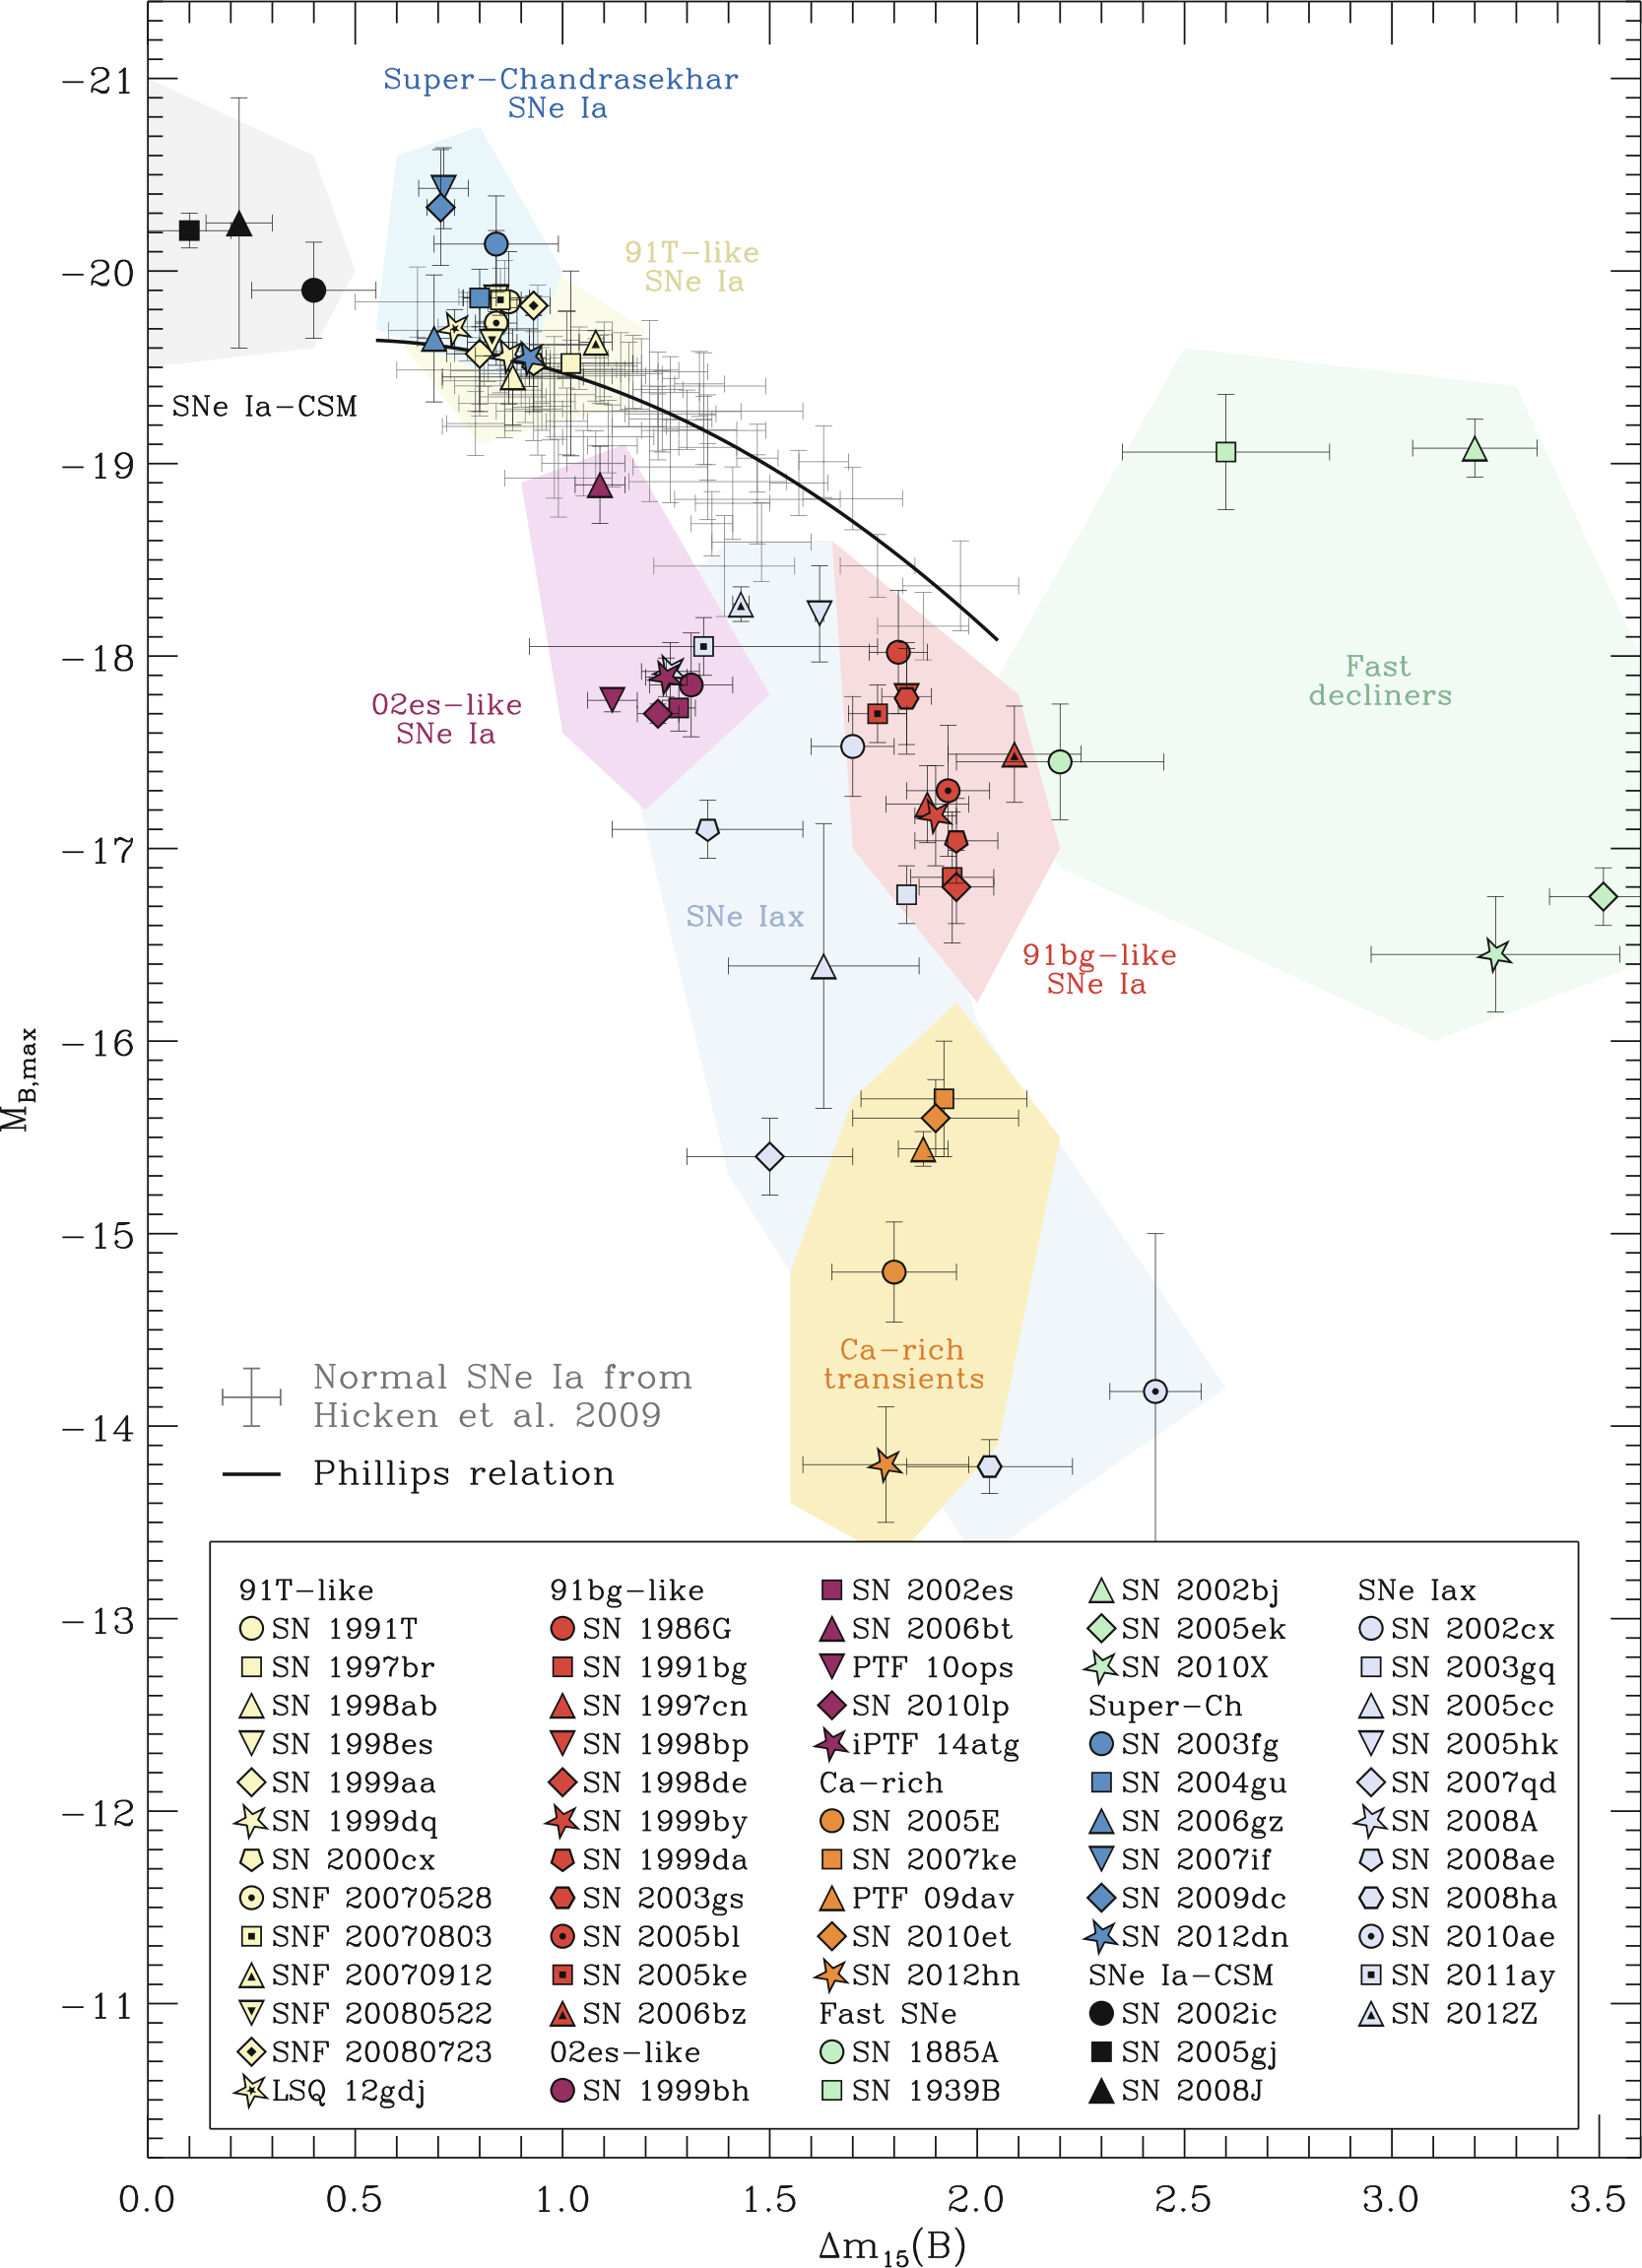
\includegraphics[width=\textwidth]{../Images/chapter_1/Taub_plot.png}
    \caption{Subclasses of SN Ia. The peak absolute B-band magnitude is plotted as a function of $\Delta m_{15}$ in the same band. Normal SNe Ia lie along the Phillips relation, which is shown with a black line. Most of the non-normal subclasses can separated from normal SNe Ia based on these two values alone. The only exception are the 91T-like SNe, which form a subclass based on their spectral differences from normal SNe Ia. This figure was taken from \citet{Taubenberger_plot}.}
    \label{Taub_plot}
\end{figure}

Recently, \citet{DR2_diversity} made a similar plot but in the \ztfg-band, using the carefully curated sample of SNe Ia from the Zwicky Transient Facility's second data release \citep[ZTF SN Ia DR2,][Smith et al., in prep.]{DR2_Overview}. They show that $\sim75$\% of all SNe Ia are normal events that can be standardized and used for distance measurements. After that the two largest subclasses are SN Ia-91T ($\sim12$\%) and SN Ia-91bg ($\sim6$\%), leaving a final $\sim7$\% as the combined total of various other subclasses of SNe.

Different subclasses have a preference for different environments. By studying the various different subclasses, the characteristic properties of their light, and the connection to their environments, we can learn more about the properties of their progenitor systems and the exact mechanisms that are involved in SN Ia explosions.


\subsection{Photometric differences}
The Phillips relation is easily visible in Figure \ref{Taub_plot}, and SNe Ia-norm lie in a narrow strip around it. Most subclasses can be distinguished from SNe Ia-norm by photometry alone. The (aptly named) fast decliners fade unusually quickly after reaching peak brightness, while SNe Ia-CSM barely fade at all in the first few weeks after reaching their peak brightness. SNe Iax never reach the peak brightness of a normal SN Ia, which in some models is explained through the explosion failing to fully disrupt the WD \citep{Iax_model_1, Iax_model_2}. Super-Chandrasekhar SNe Ia on the other hand are brighter than what would be expected from a $M_\text{Ch}$ WD explosion. Many subclasses are named after a prototypical SN that defines the subclass.


\subsection{Spectroscopic differences}
Besides photometric differences, most subclasses are also spectroscopically different from SNe Ia-norm. Some have stronger emission lines of particular elements, others have weaker ones. Ca-rich transients \citep[e.g.][]{Ca-rich_2010, Ca_rich_2012, Ca-rich_rate} show \CaII\ emission lines in their nebular spectra that are much stronger than for other SN Ia types. The spectra of super-Chandrasekhar SNe show that their ejecta move considerably slower compared to other subclasses, which together with their high luminosity is consistent with a double degenerate merger scenario \citep{2003fg_SuperCh, 06gz_SuperCh, 09dc_SuperCh}.

The SN Ia-91T subclass lies at the bright end of the Phillips relation, and thus cannot be identified photometrically but can therefore be normalized and used for distance measurements. Spectroscopy however reveals that this subclass evolves differently as it rises towards peak brigthness, showing a blue pseudo-continuum with two strong \FeIII\ absorption multiplets instead of intermediate mass element lines. They also have a preference for younger stellar populations \citep{Filippenko_91t, 91T}, although this preference is not seen in \citet{DR2_diversity}.


\section{SNe with circumstellar material}
The progenitor system of a SN is not completely isolated. Through various mechanisms a significant amount of material can end up close to the explosion site before the explosion occurs. This is called circumstellar material (CSM), and as it is usually originated from the progenitor system, CSM can give new insights in the history of the progenitor system and the sequence of events that led it to explode.

Ejecta from the SN explosion are expelled at high velocities and quickly catch up with the often much slower moving CSM. As the ejecta slam into the CSM shockwaves are produced and energy is deposited into the CSM, which starts to emit light of its own. This new light source alters the light curve, making it brighter and slowing or even stalling its decline. CSM interaction also shows up in the spectra as the emergence of narrow emission lines that give clues about the composition of the slower moving material. Eventually the ejecta overtake the CSM and its signal fades as the CSM is swept up.

Another way in which the presence of CSM has been inferred is through the presence of narrow absorption lines that vary with time, indicating that they evolve alongside the SN \citep[e.g., ][]{2013gh_NaID, 2014J_core_deg}. However, these absorption lines are not always seen and their behaviour varies from object to object, making it difficult to interpret them consistently. Light echoes can also provide an opportunity to study circumstellar and interstellar material, though the difficulty to geometrically separate them from the SN location, combined with their weak nature makes this only possible for SNe in the Milky Way or nearby galaxies \citep{Patat_light_echoes, Tycho_Brahe_classif, 2012cg}.


\subsection{The SN Ia-CSM subclass}
\label{Ia_CSM}
SNe Ia-02ic, or SNe Ia-CSM, are the subclass of thermonuclear explosions that show signs of CSM interaction. This often shows up as a peculiar long-lived light curve along with narrow Balmer emission lines, which is a clear indicator of this signal coming from CSM as SNe Ia are expected to be hydrogen-poor. The prototypical event, SN 2002ic, showed narrow \Halpha\ and \Hbeta\ lines, and the slowly declining light curve was found to be consistent with $\sim1.3$ $M_\odot$ of CSM \citep{02ic_H_det, Hamuy_02ic, 02ic_slow_decay, single_degen_CSM_gen}.

Currently there are several dozen known SNe Ia-CSM \citep{2005gj, Ia-CSM_Silverman, Ia-CSM_BTS}. In all cases the interaction started within two months after the explosion, leading to their (re-)classification after spectroscopic confirmation. The amount and duration of interaction varies quite significantly from one object to another. While some menbers such as SN 2018gkx and SN 2020xtq mainly feature an unusually slow decline rate, other objects such as SN 2020aekp have a plateau for several 100 d before starting to fade away slowly \citep{Ia-CSM_BTS}.

\begin{figure}
    \centering
    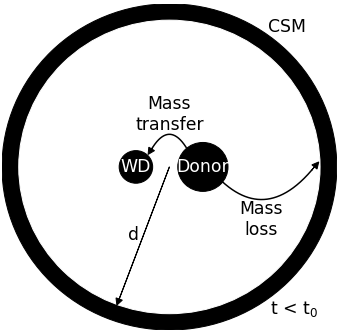
\includegraphics[height=0.281\textheight]{../Images/chapter_1/CSM_sketch_1.png}\\
    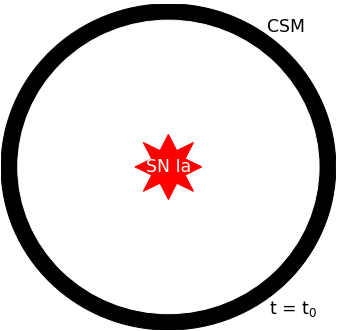
\includegraphics[height=0.281\textheight]{../Images/chapter_1/CSM_sketch_2.png}\\
    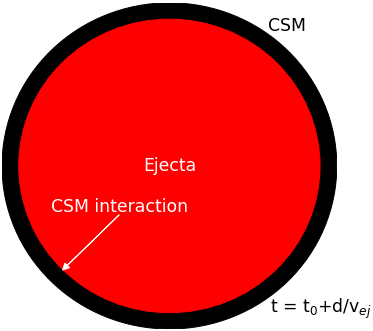
\includegraphics[height=0.281\textheight]{../Images/chapter_1/CSM_sketch_3.png}
    \caption{Schematic view of a SN Ia-CSM event. \textbf{Top:} The progenitor system containing a WD feeding on material from the donor star. Through various mechanisms a fraction of this material can be lost from the system and end up as CSM in a disk or shell at a distance $d$ around the progenitor system. \textbf{Middle:} The WD explodes as a SN Ia. This can be a SN Ia-norm or a peculiar object, depending on the progenitor system. The ejecta start traveling outwards from the explosion site. \textbf{Bottom:} The ejecta catch up to the CSM and start interacting with it, causing the CSM to start emit light as well as it is swept up. This results in a slowing down of the photometric light curve decline and narrow emission lines in the spectra. \color{red} Needs aligning \color{black}}
    \label{Ia-CSM_mod}
\end{figure}

The CSM could be created by different mechanisms depending on the progenitor system, and its composition depends on the type of donor star present. In the single degenerate scenario, CSM rich in hydrogen can be created by a WD generating a fast wind, blowing away a part of the material it received from the mass transfer \citep{single_degen_CSM_gen}. In the double-degenerate scenario, part of the tidally disrupted secondary WD becomes unbound from the system, creating (H-poor) CSM and may be able to produce detectable signatures depending on the time between the tidal disruption and the SN Ia explosion \citep{Double_degen_CSM_gen}. The core degenerate scenario could provide a massive amount of hydrogen-rich material near the explosion site \citep[e.g. for SN 2014J,][]{2014J_core_deg}, though the signatures of this scenario could be ambiguous with interacting SNe IIn, leading to confusion \citep{2012ca_Ia-CSM/IIn}. \citet{snips} proposed that the core degenerate and double degenerate scenarios could lead to SNe Ia exploding inside planetary nebulae, possibly resulting in observable time-varying sodium absorption lines or CSM interaction.

Figure \ref{Ia-CSM_mod} shows a schematic view of the creation of a CSM shell (or ring depending on how mass is lost from the progenitor system) and the subsequent interaction between the CSM and SN ejecta. When the SN explodes the ejecte will initially expand within the gap between the progenitor system and the CSM, and its spectrum will look like that of a non-interacting class of SN Ia that may or may not display absorption features caused by the CSM if it is in the line of sight. Compared to the ejecta which are traveling at $v_\text{ej}$ the CSM is practically stationary but at a distance $d$ from the explosion site. This means that the ejecta need a time $t=d/v_{ej}$ to reach the CSM and start to interact with it. Only then does the event transform into a SN Ia-CSM with new narrow emission lines. This later transformation explains why in some cases objects are re-classified as Ia-CSM after first being classified as something else (e.g. SN 2020aekp, which was first classified as a SN Ia by \citealt{2020aekp_1st_classif} but reclassified as a SN Ia-CSM by \citealt{2020aekp_reclassif}).

SN 2011km (PTF11kx) is a well observed Ia-CSM event, and shows signs of a complex CSM consisting of multiple shells with which the SN ejecta interact. \citet{ptf11kx} show that its photometry is similar to 91T-like objects before the CSM interaction begins, and explain SN 2011km using a symbiotic nova progenitor system. \citet{Ia-CSM_and_91T_connection} also suggested a link between SNe Ia-91T and SNe Ia-CSM as they show  similarities in their peak brightness and spectroscopy before the start of the interaction. In some cases, a 91T-like SN could start interacting with CSM hundreds of years after the explosion, like as has been suggested for Kepler’s SN \citet{Kepler_91T, Kepler_CSM}.

Another interesting Ia-CSM is SN 2020eyj, which \citet{Kool_He_CSM} present as the first detection of a Ia-CSM interacting with He-rich material. Up until then all members of the subclass had shown strong \Halpha\ emission and weak He signatures. SN 2020eyj, however, showed little to no H present in the CSM. This suggests that the progenitor system contained a He star. This was also the first time a SN Ia was detected in the radio. Non-detections in normal SNe Ia suggest a clean environment for the ejecta to expand in, while in this case there is a lot of material present.


\subsection{CSM in CCSNe}
Some CCSNe show interaction with CSM as well, the events are subclassified as SN IIn, SN Ibn, or SN Icn, due to the narrow emission lines. As stated in Section \ref{CCSN} the difference between these three main types of SNe is the amount of material that has been stripped prior to explosion. Mass can be lost through binary interaction, but massive stars have also been known to have strong stellar outflows and winds. The existence of Wolf-Rayet stars shows that very massive stars can lose their entire hydrogen envelope, and they are thought to be one of the very last stages in the life of the star before it explodes in a SN Ib or SN Ic \citep{WR_as_progenitors, 2019hgp}.

The CSM is often resides close to the progenitor and can be thick enough to obscure features of the underlying SN, depending on the geometry and orientation of the system \citep{1994W, PTF11iqb}. The short distance between the SN and CSM suggest that the material was ejected recently, and in some cases precursor events have been observed prior to the final SN explosion (e.g. SN 2011ht, \citealt{2011ht} and SN 2020pvb \citealt{2020pvb}). CSM residing close to the progenitor causes most CCSNe to show signs of CSM interaction almost immediately after the explosion. However, examples of the interaction starting much later have been found as well, suggesting that their CSM has been ejected a long time ago \citep{2008iy, late-CSM_IIn_Spitzer}.

Recently, SN 2021yfj was discovered to be a new type of SN and given the classification of SN Ien. This object showed highly ionized silicon, sulpher, and argon lines but barely any carbon, oxygen, helium, or hydrogen. This suggests the progenitor being a massive star stripped all the way down to its final layer before the iron core. The classification leaves space for the yet to be discovered explosion of a slightly less stripped star in a SN Type Idn which would have no carbon but strong oxygen, neon, and magnesium emission lines, as well as their non-interacting counterparts and transitional objects. \citep{Ien_disc}. \color{red} Get astronote ref in ones its on ADS \color{black}


\subsection{Distant CSM}
As stated in Section \ref{Ia_CSM} and shown in Figure \ref{Ia-CSM_mod}, there is a delay between the SN explosion and the start of CSM interaction due to the distance between the progenitor system and CSM. All objects that are currently classified as SNe Ia-CSM on the Transient Name Server\footnote{https://www.wis-tns.org/} (TNS) have shown signs of interaction at or around peak brightness. Assuming an ejecta velocity of $v_\text{ej} \sim 20\,000$ km s$^{-1}$ and that the interaction starts on average around the SN peak $\sim3$ weeks after the explosion, the CSM is located at a distance $d\sim3.5\times10^{15}$ cm of the progenitor system \citep{Ia-CSM_BTS}. If however the CSM is at a distance of $d\sim10^{17}$ cm, ejecta with the same $v_\text{ej}$ would need $\sim1.5$ years to catch up and start interacting.

In the effort to systematically search for such late-time CSM interaction, \citet{2015cp} looked at old ($\geq1$ year) SNe using the \textit{Hubble Space Telescope} (HST). They focused their search on subclasses, such as 91T, that are associated with CSM interaction \citep{Ia-CSM_and_91T_connection}. Out of 72 targets, only ASASSN-15og and SN 2015cp were found to show late-time CSM interaction. ASASSN-15og is a Type IIn SN with detected CSM interaction around peak, and was used as a control object. SN 2015cp has been classified as a 91T-like SN Ia, without signs of CSM interaction around peak. This showed that late-time CSM interaction may be systematically missed due to SNe Ia not being actively followed at these phases. From a progenitor point of view this means that material can be ejected from the system prior to the explosion, giving it time to travel further before being caught up by the SN ejecta.

\citet{GALEX_Late_CSM} used archival UV-band data from the \textit{Galactic Evolution Explorer} (GALEX) to look for late-time CSM interaction in SNe Ia. Out of a sample of 1080 SNe Ia, 4 were detected in the UV near peak, but none showed signs of late-time CSM interaction. They show that this type of CSM interaction is rare, occurring between 500 to $1\,000$ d after the initial discovery of the SN in $<5$\% of the SNe Ia at a strength similar to SN 2015cp, and a decreasing percentage as the interaction gets stronger. \color{red} Make sure all mentions of full spacecraft names are in italics \color{black}



\section{In this thesis:...}
In this thesis I will present my work on the search for signs of late-time interaction in Type Ia SNe using observations taken by ZTF survey. In Chapter \ref{chap:obs} I will introduce the survey as well as the other facilities that have been used to gather data that is presented in this thesis. I will also give an overview of the basics of observing, some of the types of data that can be obtained, and the basic steps that are required to reduce them to something that can be used in further analysis.

Chapter \ref{chap:DR2_search} is an adaptation of \cite{Terwel_2024_paper1}, and presents my search for late-time signals in the ZTF SN Ia DR2, which consists of $3\,628$ spectroscopically classified SN Ia that were first discovered between March 2018 and October 2020. It also details the pipeline and analysis tools I developed to search in a consistent manner (Section \ref{DR2_analysis}).

It might be possible that a late-time signal is observed by ZTF while the main transient occured before the survey started. In Chapter \ref{chap:pre-ZTF_search} I search for this type of event using a slightly modified version of the pipeline used for the DR2 search. As the analysis is exactly the same whether the original transient was a SN Ia, SN II, or any other type of transient, I search through a sample of 8707 transients that were first discovered between 1 January 2008 and 1 January 2018.

Up to this point my search has been through archival data only, with the obvious drawback that it is very likely that any recovered late-time signal cannot be followed up on. By further modifying the pipeline I search in Chapter \color{red} not put in yet \color{black} for late-time signals in SNe Ia in real-time using the latest ZTF observations with the goal to follow up photometrically and/or spectroscopically using other telescopes.

Finally, in Chapter \color{red} not put in yet \color{black} I conclude on the results of searching through these three samples and finish with possible continuations of this search, modifications, and possible alternative usages for this or a similar pipeline.

To convert between apparent and absolute magnitude I assume a flat $\Lambda$CDM cosmology with H$_0 = 67.7$ km s$^{-1}$ Mpc$^{-1}$ and $\Omega_\text{m} = 0.310$ \citep{Planck18VI} throughout this thesis, unless specified otherwise. \color{red} Do I use another one anywhere? \color{black}

\end{document}